\chapter{Artificial Intelligence}

\section{Knowledge Representation}

\begin{defi}[Belief change scenario]
A \term{belief change scenario} is a triple $B=\tuple{K,R,C}$, where $K$, $R$ and $C$ are sets of formula over a fixed propositional language $\calLcalP$. Informally, $K$ is a \term{knowledge base} which is to be modified in such a way that the resulting knowledge base includes all elements from $R$ and does not include any element from $C$. The modified knowledge base corresponding to $B$ will be denoted by $K\dotplus R\dotminus C$.
\cite{conf/fedcsis/KorpusikLM12}
\end{defi}

\begin{defi}[Belief change extension, Unique (inconsistent) belief change extension]
Let $B=\tuple{K,R,C}$ be a belief change scenario over $\calLcalP$. Define a new set $\calP'$ of atoms, isomorphic with $\calP$, given by $\calP'=\accol{p':p\in\calP}$. Let $K'$ be a knowledge base obtained from $K$ by replacing any $p\in\calP$ by $p'\in\calP'$. Let $EQ$ be a maximal (with respect to set inclusion) set of equivalences $\accol{p\Leftrightarrow p'|p\in\calP}$ such that $\fun{Th}{K'\cup EQ\cup R}\cap\brak{C\cup\bot}=\emptyset$. The set $\fun{Th}{K'\cup EQ\cup R}\cap\calLcalP$ is called a \term{belief change extension} of $B$. If there is no such set $EQ$, then $B$ is inconsistent and $\calLcalP$ is a \term{unique (inconsistent) belief change extension} of $B$.
\cite{conf/fedcsis/KorpusikLM12}
\end{defi}

\begin{defi}[Class of all belief change extensions]
Let $\accol{E_i}_{i\in I}$ be the \term{class of all belief change extensions} of $B=\tuple{K,R,C}$. Then
\begin{equation}
K\dotplus R\dotminus C=\displaystyle\bigcap_{i\in I}E_i
\end{equation}
\cite{conf/fedcsis/KorpusikLM12}
\end{defi}

\begin{defi}[Knowledge base, Observation, Defeasible statement, Domain axiom]
A \term{knowledge base} is a triple $KB=\tuple{OB,DS,DA}$, where $OB$, $DS$ and $DA$ are finite sets of formulas. These sets are referred to as \term{observation}s, \term{defeasible statement}s and \term{domain axiom}s, respectively.
\cite{conf/fedcsis/KorpusikLM12}
\end{defi}

\begin{defi}[Revision formula, Revision]
Let $KB=\tuple{OB,DS,DA}$ be a knowledge base and suppose that $\alpha$ is a \term{revision formula} representing a new observation. A \term{revision} of $KB$ by $\alpha$, written $KB\ast\alpha$, is a new knowledge base given by $\tuple{OB_1,DS,DA}$, where $OB_1=OB\oplus\accol{\alpha}\ominus\accol{\neg DA\hat{}}$. Here $\accol{\alpha}\ominus\accol{\neg DA\hat{}}$ is a finite representation of the modified knowledge base corresponding to belief change scenario $\tuple{OB,\accol{\alpha},\accol{\neg DA\hat{}}}$.
\cite{conf/fedcsis/KorpusikLM12}
\end{defi}

\begin{defi}[Belief set corresponding to]
Let $KB=\tuple{OB,DS,DA}$ be a knowledge base. A \term{belief set corresponding to} $KB$, written $B_{KB}$, is given
by $DS\dotplus\brak{OB\cup DA}$.
\cite{conf/fedcsis/KorpusikLM12}
\end{defi}

\begin{defi}[Prioritized belief revision of $KB$ by $\alpha$]
Let $KB=\tuple{OB,DS,DA}$ be a knowledge base and $\alpha$ be a revision formula. Let $OB_1=OB\oplus\accol{\alpha}\ominus\accol{\neg DA\hat{}}$. The \term{prioritized belief revision of $KB$ by $\alpha$} with respect to priorities $DS_1<DS_2<\ldots<DS_n$, written $KB\ast^{\flatbrak{DS_1<DS_2<\ldots<DS_n}}\alpha$, is the formula
\begin{equation}
DS_1\dotplus\brak{DS_2\oplus\ldots\brak{DS_n\oplus (OB_1\cup DA)\ldots}}.
\end{equation}
\cite{}
\end{defi}

\begin{defi}[Closure of a knowledge base]
Let $*CW\ A$ be any closed world assumption policy among (basic) Closed World Assumption (CW A), Generalized Closed World Assumption (GCW A), Extended Generalized Closed World Assumption (EGCW A), Careful Closed World Assumption (CCW A) and Extended Closed World Assumption (ECW A). Let $\Sigma$ be a formula from $\mbox{PROP}_{\mbox{PS}}$ and $\tuple{P,Q,Z}$ a partition of $\fun{\mbox{Var}}{\Sigma}$. The \term[Closure of a knowledge base]{closure} $\fun{*CW\ A}{\Sigma,\tuple{P,Q,Z}}$ of $\Sigma$ given $\tuple{P,Q,Z}$ \wrtTx{} $*CW\ A$ is the formula $\Sigma\cup\accol{\neg\alpha|\alpha\mbox{ is a $*CW\ A$-free for negation formula \wrtTx{} $\Sigma$ and $\tuple{P,Q,Z}$}}$.
\cite{conf/ijcai/Coste-MarquisM99}
\end{defi}

\begin{defi}[Closed World Assumption-free for negation formula]
Let $\Sigma$ and $\alpha$ be two formulas from $\mbox{PROP}_{\mbox{ps}}$ and let $\tuple{P,Q,Z}$ be partition of $\fun{\mbox{Var}}{\Sigma}$. $\alpha$ is \termabbrev{Closed World Assumption-free}{CW A-free} for negation \iffTx{} $\alpha$ is a positive literal \stTx{} $\Sigma\nvDash\alpha$ holds.
\cite{conf/ijcai/Coste-MarquisM99}
\end{defi}

\begin{defi}[Generalized Closed World Assumption-free for negation formula]
Let $\Sigma$ and $\alpha$ be two formulas from $\mbox{PROP}_{\mbox{ps}}$ and let $\tuple{P,Q,Z}$ be partition of $\fun{\mbox{Var}}{\Sigma}$. $\alpha$ is \termabbrev{Generalized Closed World Assumption-free}{GCW A-free} for negation \iffTx{} $\alpha$ is a positive literal and for each positive clause $\gamma$ \stTx{} $\Sigma\nvDash\gamma$ holds, $\Sigma\nvDash\alpha\vee\gamma$ holds.
\cite{conf/ijcai/Coste-MarquisM99}
\end{defi}

\begin{defi}[Extended Generalized Closed World Assumption-free for negation formula]
Let $\Sigma$ and $\alpha$ be two formulas from $\mbox{PROP}_{\mbox{ps}}$ and let $\tuple{P,Q,Z}$ be partition of $\fun{\mbox{Var}}{\Sigma}$. $\alpha$ is \termabbrev{Extended Generalized Closed World Assumption-free}{EGCW A-free} for negation \iffTx{} $\alpha$ is a conjunction of positive literals and for each positive clause $\gamma$ \stTx{} $\Sigma\nvDash\gamma$ holds, $\Sigma\nvDash\alpha\vee\gamma$ holds.
\cite{conf/ijcai/Coste-MarquisM99}
\end{defi}

\begin{defi}[Careful Closed World Assumption-free for negation formula]
Let $\Sigma$ and $\alpha$ be two formulas from $\mbox{PROP}_{\mbox{ps}}$ and let $\tuple{P,Q,Z}$ be partition of $\fun{\mbox{Var}}{\Sigma}$. $\alpha$ is \termabbrev{Careful Closed World Assumption-free}{CCW A-free} for negation \iffTx{} $\alpha$ is a literal from $L_P^+$ and for each clause $\gamma$ containing only literals from $L_P^+\cup L_Q$  and \stTx{} $\Sigma\nvDash\gamma$ holds, $\Sigma\nvDash\alpha\vee\gamma$ holds.
\cite{conf/ijcai/Coste-MarquisM99}
\end{defi}

\begin{defi}[Extended Closed World Assumption-free for negation formula]
Let $\Sigma$ and $\alpha$ be two formulas from $\mbox{PROP}_{\mbox{ps}}$ and let $\tuple{P,Q,Z}$ be partition of $\fun{\mbox{Var}}{\Sigma}$. $\alpha$ is \termabbrev{Extended Closed World Assumption-free}{ECW A-free} for negation \iffTx{} $\fun{\mbox{Var}}{\alpha}\cap Z=\emptyset$ and for each clause $\gamma$ containing only literals from $L_P^+\cup L_Q$  and \stTx{} $\Sigma\nvDash\gamma$ holds, $\Sigma\nvDash\alpha\vee\gamma$ holds.
\cite{conf/ijcai/Coste-MarquisM99}
\end{defi}

\begin{defi}[*CWA clause inference, *CWA literal inference]
Let $*CWA$ be any closed world assumption policy among (basic) Closed World Assumption (CW A), Generalized Closed World Assumption (GCW A), Extended Generalized Closed World Assumption (EGCW A), Careful Closed World Assumption (CCW A) and Extended Closed World Assumption (ECW A).  \term{*CWA clause inference} is the following decision:
\begin{enumerate}
 \item Input: A formula $\Sigma$ and clause $\gamma$ from $\mbox{PROPS}_{\mbox{PS}}$, a partition $\tuple{P,Q,Z}$ of $\funm{Var}{\Sigma}$ and a CWA policy $*CWA$
 \item Query: Does $\fun{*CW\ A}{\Sigma,\tuple{P,Q,Z}}\vDash\gamma$ holds?
\end{enumerate}
\term{*CWA literal inference} is the restriction of the corresponding $*CWA$ clause inference problem where $\gamma$ is restricted to be a literal.
\cite{conf/ijcai/Coste-MarquisM99}
\end{defi}

\begin{defi}[Blake formula]
Let $\Sigma$ be a formula from $\mbox{PROP}_{\mbox{PS}}$. $\Sigma$ is a \term{Blake formula} \iffTx{} $\Sigma$ is a CNF formula and for every implicate $\gamma$ of $\Sigma$, there exists a clause $\pi$ in $\Sigma$ \stTx{} $\pi\vDash\gamma$ holds.
\cite{conf/ijcai/Coste-MarquisM99}
\end{defi}

\begin{defi}[Disjunct normal form formula]
Let $\Sigma$ be a formula from $\mbox{PROP}_{\mbox{PS}}$. $\Sigma$ is a \termabbrev{Disjunction normal form formula}{DNF formula} \iffTx{} $\Sigma$ is a finite disjunction of terms.
\cite{conf/ijcai/Coste-MarquisM99}
\end{defi}

\begin{defi}[Horn cover formula]
Let $\Sigma$ be a formula from $\mbox{PROP}_{\mbox{PS}}$. $\Sigma$ is a \term{Horn cover formula} \iffTx{} $\Sigma$ is a finite disjunction of Horn CNF formulas.
\cite{conf/ijcai/Coste-MarquisM99}
\end{defi}

\begin{defi}[Renamable Horn cover formula]
Let $\Sigma$ be a formula from $\mbox{PROP}_{\mbox{PS}}$. $\Sigma$ is a \term{renamable Horn cover formula} \iffTx{} $\Sigma$ is a finite disjunction of renamable Horn CNF formulas.
\cite{conf/ijcai/Coste-MarquisM99}
\end{defi}

\begin{defi}[Finite representation of the modified knowledge base corresponding to belief change scenario]
Let $KB=\tuple{OB,DS,DA}$ and suppose that $\alpha$ is a revision formula representing a domain axiom. The revised knowledge base is defined by $KB\ast\alpha=\tuple{OB1,DS,DA\cup\accol{α}}$, where $OB_1=OB\oplus\accol{\top}\ominus\accol{\neg\brak{DA\cup\accol{\alpha}}\hat{}}$. Here $OB\oplus\accol{\top}\ominus\accol{\neg\brak{DA\cup\accol{\alpha}}\hat{}}$ is a \term{finite representation of the modified knowledge base corresponding to belief change scenario}, $\tuple{OB,\accol{\top},\accol{\neg\brak{DA\cup\accol{\alpha}}\hat{}}}$.
\cite{conf/fedcsis/KorpusikLM12}
\end{defi}

\begin{defi}
Let $KB=\tuple{OB,DS,DA}$ and suppose that $\alpha$ is a revision formula representing a defeasible statement. The revised knowledge base is defined by $KB\ast\alpha=\tuple{OB,DS_1,DA}$, where $DS_1=DS\oplus\accol{\alpha}$.
\cite{conf/fedcsis/KorpusikLM12}
\end{defi}

\section{Optimization Problems}

\begin{defi}
A \term{neighborhood structure} is a function $\calN:\calS\rightarrow 2^\calS$ that assigns to every $s\in\calS$ a set of neighbors $\fun{\calN}{s}\subseteq\calS$. $\fun{\calN}{s}$ is called the neighborhood of $s$. Often, neighborhood structures are implicitly defined by specifying the changes that must be applied to a solution s in order to generate all its neighbors. The application of such an operator that produces a neighbor $s'\in\fun{\calN}{s}$ of a solution s is commonly called a \term{move}.\cite{alba05}
\end{defi}

\begin{defi}
A \term{locally minimal solution} (or \term{local minimum}) with respect to a neighborhood structure $\calN$ is a solution $\hat{s}$ such that $\forall s\in\neigh{\hat{s}}:\ffun{\hat{s}}\leq\ffun{s}$. We call $\hat{s}$ a \term{strict locally minimum} if $\forall s\in\neigh{\hat{s}}:\ffun{\hats}<\ffun{s}$.\cite{alba05}
\end{defi}

\section{Toxicology}

\begin{defi}[Performance comparison]
The predictive accuracies of two theories are statistically equivalent then the theory with better explanatory power has \term[Performance comparison]{better performance}. Otherwise the one with higher accuracy has better performance.
\cite{conf/ijcai/SrinivasanKMS97}
\end{defi}

\section{Production Systems}

\begin{defi}[Object pattern, Object body, Object instance]
An \term{object pattern} is an $n$-tuple with an \term{object body}. It has the following format:
\begin{equation}
\fun{OP}{x_1,x_2,\ldots,x_n}:\mbox{object body}
\end{equation}
where $OP$ is the calss-name of this object pattern and $x_i$ is the value of the $i$-th attribute in $OP$, and $x_i$ must meet some constraint $C_i$. An object body is an associated list composed of object calss and attribute-value pairs. It has the following format:
\begin{equation}
\tuple{\mbox{object-class}\ \hat{}\mbox{attr}_1\ \mbox{value}_1\ \hat{}\mbox{attr}_2\ \mbox{value}_2\ \hat{}\ldots\ \hat{}\mbox{attr}_n\ \mbox{value}_n}
\end{equation}
where $\mbox{value}_i$ can be a constant or a variable with some constraint. Let \fun{P}{x_1,x_2,\ldots,x_n} be an object body, then we call \fun{P}{c_1,c_2,\ldots,c_n} is an \term{object instance} of $P$, where $c_i$ is a constant and must meet the constraint of $\mbox{value}_i$. Its instance body is
\begin{equation}
\tuple{\mbox{object-class}\ \hat{}\mbox{attr}_1\ c_1\ \hat{}\mbox{attr}_2\ c_2\ \hat{}\ldots\ \hat{}\mbox{attr}_n\ c_n}
\end{equation}
\fun{I}{P} denotes the set of all possible object instances of object pattern $P$.
\cite{conf/ijcai/HsuW89}
\end{defi}

\begin{defi}[Precondition set of a rule]
The \term[Precondition set of a rule]{precondition set $\mbox{PRESET}_i$ of a rule $i$} is a set of marked object patterns, i.e., the condition elements (positively/negatively referenced) in the left-hand side of rule $i$. If an object pattern $C_j$ is positively referenced, then it will be marked as $+C_j$ in $\mbox{PRESET}_i$; if negatively referenced, then marked as $-C_j$.
\cite{conf/ijcai/HsuW89}
\end{defi}

\begin{defi}[Changed set of a rule]
The \term[Changed set of a rule]{changed set $\mbox{CHANGE}_i$ of a rule $i$} is a set of marked object patterns, i.e., the added or deleted object patterns in the right-hand side of rule $i$. If an object pattern $W_i$ is added by a make action, then it will be marked as $+W_j$ in $\mbox{CHANGE}_j$ ; if deleted by a remove or a modify action, then marked as $-W_j$.
\cite{conf/ijcai/HsuW89}
\end{defi}

\begin{defi}[Rule having interference dependency on another rule]
\term[Rule having interference dependency on another rule]{Rule $r_i$ has an interference dependency on rule $r_j$}\tabbrev{Rule having interference dependency on another rule}{I-DEP} \iffTx{} the set formed by all the naged instances of the changed set of rule $r_i$ and the set formed by all the instances of the precondition set of rule $r_j$ are disjoint. That is,
\begin{equation}
\fun{\neg I}{\mbox{CHANGE}_i}\cap\fun{I}{\mbox{PRESET}_j}=\emptyset
\end{equation}
Let IN be the set formed as follows:
\begin{equation}
\mbox{IN}=\accol{p|p\in\mbox{PRESET}_j,\fun{I}{p}\cap\fun{\neg I}{\mbox{CHANGE}_i}=\emptyset}
\end{equation}
Where $\fun{\neg I}{\mbox{CHANGE}_i}$ means to negate the elements in $\fun{I}{\mbox{CHANGE}_i}$, i.e., \funm{added}{\mbox{deleted}} object pattern will become \funm{deleted}{\mbox{added}}. If rule $r_i$ has an inference dependency on rule $r_j$ \wrtTx{} the set $IN$, then in the i-dependency augmented digraph, there exists one subdigraph shown in figure \ref{fig:subdigraphin}.
\cite{conf/ijcai/HsuW89}
\end{defi}

\begin{figure}[hbt]
\centering
\subfigure[Inference dependency]{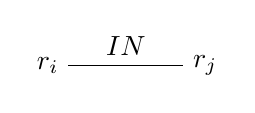
\begin{tikzpicture}
\node (ri) at (0,0) {$r_i$};
\node (rj) at (2,0) {$r_j$};
\draw (ri) to node[above,midway] {$IN$} (rj);
\end{tikzpicture}
\label{fig:subdigraphin}}
\subfigure[Input-output]{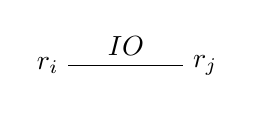
\begin{tikzpicture}
\node (ri) at (0,0) {$r_i$};
\node (rj) at (2,0) {$r_j$};
\draw (ri) to node[above,midway] {$IO$} (rj);
\end{tikzpicture}
\label{fig:subdigraphio}}
\caption{Subdigraphs in the i-dependency and io-dependency augmented digraph.}
\end{figure}


\begin{defi}[Rule having input-output dependency on another rule \wrtTx{} a set]
\term[Rule having input-output dependency on another rule \wrtTx{} a set]{Rule $r_i$ has an input-output dependency on rule $r_j$ \wrtTx{} a set $IO$}\tabbrev{Rule having input-output dependency on another rule \wrtTx{} a set}{IO-DEP} \iffTx{}
\begin{equation}
\fun{I}{\mbox{CHANGE}_i}\cap\fun{I}{\mbox{PRESET}_j}=\emptyset
\end{equation}
Where $IO=\accol{p|p\in\mbox{PRESET}_j\wedge\fun{I}{P}\cap\fun{I}{\mbox{CHANGE}_i}=\emptyset}$. If rule $r_i$ has an input-output dependency on rule $r_j$ \wrtTx{} the set $IO$, then in the io-dependency augmented digraph, there exists one subdigraph shown in figure \ref{fig:subdigraphio}.
\cite{conf/ijcai/HsuW89}
\end{defi}

\begin{defi}[Following rule set of a rule]
The \term{following rule set of a rule} $r$, \funm{Follow}{r}, is the set of all rules that are reachable from rule $r$ in the io-dependency augmented digraph unioned with the rule $r$ itself.
\cite{conf/ijcai/HsuW89}
\end{defi}

\begin{defi}[Descent rule of another rule]
If rule $r\in\funm{Follow}{r_i}$, then we call rule $r$ a \term{descent rule} of $r_i$.
\cite{conf/ijcai/HsuW89}
\end{defi}

\begin{defi}[Rule having an inference relation on another rule]
\term[Rule having an inference relation on another rule]{Rule $r_i$ has an inference relation on rule $r_j$} \tabbrev{Rule having an inference relation on another rule}{I-R} if there exists at least one rule $r\in\funm{Follow}{r_i}$ \stTx{} rule $r$ has an I-DEP on rule $r_j$ or rule $r_j$ has an I-DEP on rule $r$.
\cite{conf/ijcai/HsuW89}
\end{defi}

\begin{defi}[Derivation step, Derivation sequence]
Let $G_0$ be a set of object instantiations. We call $G_0\rightarrow^r G_1$ a \term{derivation step} if:
\begin{enumerate}
 \item for all $p\in\mbox{PRESET}_r$, if $p$ is marked $+$ and there exists one element $x$ of \fun{I}{p}, \stTx{} $x\in G_0$, or if $p$ is marked $-$, and \faTx{} $x$ in \fun{I}{p}, $x$ is not in $G_0$, and
 \item $G_1=G_0+\fun{A}{r}-\fun{D}{r}$ where \fun{A}{r} is the set of all object instances added by rule $r$, and \fun{D}{r} is the set of all object instances deleted by rule $r$. And let \fun{ILHS}{r} be the set of positive marked object instances, then \fun{D}{r} is a subset of \fun{ILHS}{r}.
\end{enumerate}
If $G_0\rightarrow^{r_1}G_1\rightarrow^{r_2}\ldots\rightarrow^{r_n}G_n$ we call $r_1\rightarrow r_2\rightarrow\ldots\rightarrow r_n$ a \term{derivation sequence}, which can be denoted by $r^{\star}$, then: $G_0\rightarrow^{r^{\star}}G_n$.
\cite{conf/ijcai/HsuW89}
\end{defi}

\begin{defi}[Equivalent derivation sequences]
Two derivation sequences $r_1^{\star}$ and $r_2^{\star}$ are called \term[Equivalent derivation sequences]{equivalent} if:
\begin{equation}
G_0\rightarrow^{r_1^{\star}}G_n\wedge G_0\rightarrow^{r_2^{\star}}G_m\wedge G_n=G_m
\end{equation}
The relation is denoted as $r_1^{\star}=r_2^{\star}$.
\cite{conf/ijcai/HsuW89}
\end{defi}